\documentclass[12pt]{article}
\usepackage[utf8]{inputenc} 
\usepackage[T1]{fontenc}
\usepackage{amssymb}
\usepackage{amsmath}
\usepackage[francais]{babel} 
\usepackage[top=2cm, bottom=2cm, left=2cm, right=2cm]{geometry}
\usepackage{setspace}
\usepackage{listings}
\usepackage{caption}
\usepackage{subcaption}
\usepackage{sidecap}
\usepackage{pdfpages}
\usepackage{sidecap}
\usepackage{multicol}
\usepackage{titlesec}
\usepackage{enumitem}
\setlist[itemize]{noitemsep}
\usepackage{xcolor}
\usepackage{mdframed}
\usepackage{hyperref}
\newmdenv[%
    leftmargin=-5pt,
    rightmargin=-5pt, 
    innerleftmargin=5pt,
    innerrightmargin=5pt,
    backgroundcolor=brown!10,
]{Answer}%



\begin{document}
\makeatletter
\thispagestyle{empty}
	\begin{center}
		\vspace*{-1cm}
		\noindent\hrulefill
		\vspace{0.5cm}
		
		\begin{minipage}[c]{0.7\textwidth}
			\bf\Large\centering
			RM01 - Option A - Examined Assignment Question 1\end{minipage}

		\vspace{0.5cm}
		\noindent\hrulefill	
		\vspace{0.5cm}
		
		{
			LE456, January 2018
			\vspace{0.5cm}			
		}
	\end{center}
\makeatother

\section{Introduction}

The housing wealth effect, however controversial in certain cases (Buiter, 2008; Calomiris et al., 2009), corresponds to the positive relationship between perceived housing wealth and consumption (Case et al., 2005; Carroll et al., 2011). Said effect and its relationship to energy consumption will be investigated within the given dataset.\\

Before going any further, can we first deduce what kind of model would we expect ? What variables and factors would one expect to be relevant to this question ? Surely physical characteristics of the house would be of key importance (e.g. its size, the number of persons living in it, the time spent in the house, the thermic isolation). Obviously, the economics of the household would as well, as directly influencing the possible amount of money spendable on energy consumption (e.g. household total income, future financial perspective). Additionally, some behavioural factors, which could be described as socio-cultural, have been shown to be quite crucial (e.g. education, environmental awareness or the use of dwelling appliances). Finally, the climate and outside temperatures would not have the least effect. \\

One would therefore expect a model as follows:\\

$Consumption_{i} = Intercept + Climate_i + House_i + Economics_i + SocioCultural_i + E_{i}$ with $ E_{i} \sim \mathcal{N}(0,\sigma^2)$ and $i$ the household.\\

Which one would want to compare to:\\
$Consumption_{i} = Intercept + HousingWealth_i +Climate_i + House_i + Economics_i + SocioCultural_i + E_{i}$\\

With that in mind, I will first perform a preliminary data analysis, which includes data selection and transformation, followed by the models construction and evaluation and, finally, results well be further interpreted and discussed. \\

All analysis were performed on R version 3.3.2 and the source scripts are available on Github (http://bit.ly/2DqV0B1).\\

\section{Preliminary Data Analysis}
\subsection{Sorting variables}

Before any further considerations, variables were carefully assessed and sorted by categories. Based on previous readings and interpretations as well as arbitrary judgements the variables were sorted as follows:
\begin{enumerate}
\item $Y$ (Response variable: $FUELANNUAL$). The annual spending of combined gas and electricity is the proxy for energy consumption.
\item $X$ (Explaining variable of interest: $HSVAL$). The amount of money for which the respondents would expect to sell their house is the proxy for perceived housing wealth.
\item $Dynamics$ (Explaining variables related to regional and yearly dynamics).
\item $Household$ (Explaining variables related to the households size and composition). Notably, there is no direct size measure of the house, indirect indication however are included, such as the number of bedrooms.
\item $Economics$ (Explaining variables related to the households economics). This includes, for instance, information such as the gross monthly income of the household.
\item $Cultural$ (Explaining variables related to the households cultural characteristics). That category takes into account factors such as education level.
\item $Environmental$ (Explaining variables related to the households environmental behaviour). This uses the results of energy consumption behaviours.
\item $Fuel \& Heating$ (Explaining variables related to the households fuel bills and heating). This final category includes specificities such as separate bills between gas and electricity or the presence of central heating systems.
\end{enumerate}

\subsection{Dealing with missing values}
After a first glimpse of dataset, the need to deal with missing values appear to be obvious. Due to the consequent size of the dataset (4534 observations) I choose a rather conservative way of approaching the issue. Firstly, all observations (rows) with missing values in either $FUELANNUAL$ or $HSVAL$ were removed, as they do not contain the variables of interests. Subsequently, the rest of the variables were pre-selected based on the number of missing observations. Figure 1 indicates three main group of variables, with either less than 15\% of missing values, roughly between 35 and 50\% and finally more than 65\%. Only the first category of variables was kept in order to maximise the number of observations. However, a sanity check was subsequently performed in order to ensure that no key information was dropped in the process.

\begin{figure}[!h]
\begin{center}
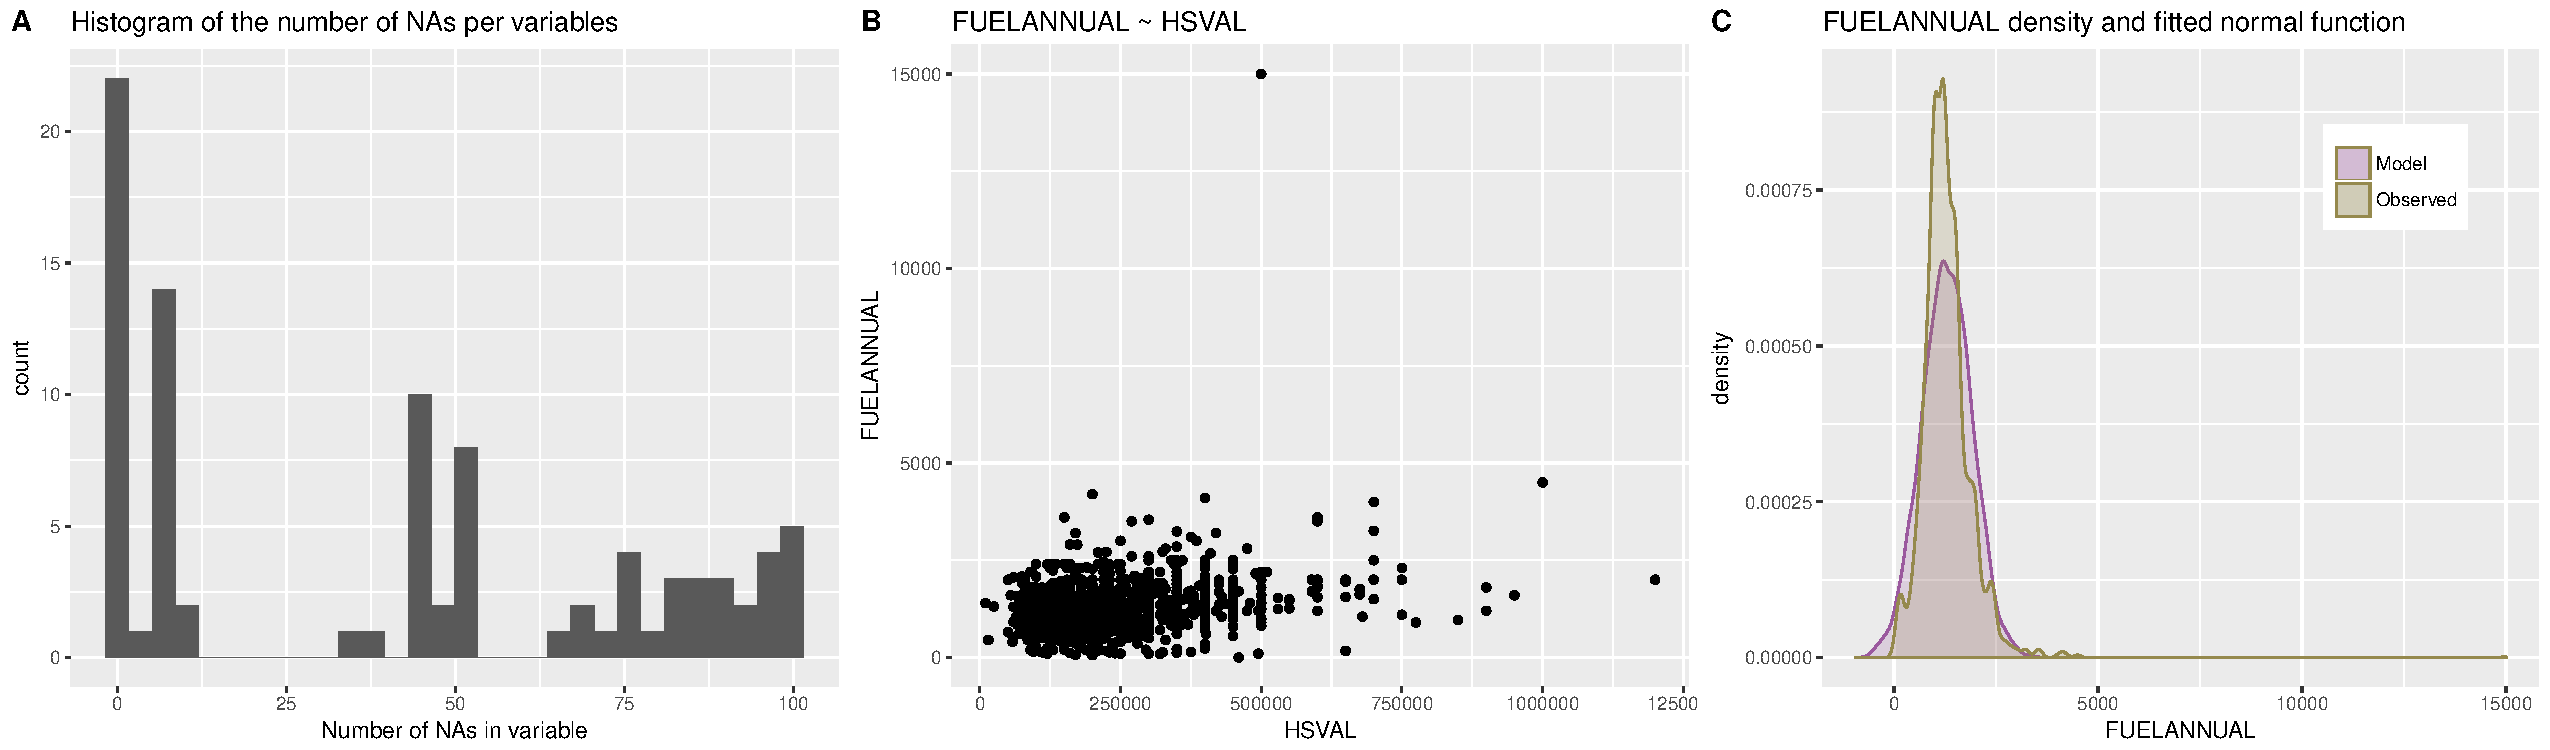
\includegraphics[width=17cm]{../Figure_NAs.pdf}
\end{center}
\caption{\footnotesize{A - Distributions of NAs across the variables; B - Biplot of FUELANNUAL as a function of HSVAL; C - density functions (observed and modelled) of FUELANNUAL}}
\label{Figure 1}
\end{figure}

In the end, remaining missing values from selected variables were removed. Leading to a total of 2193 observations, 76.3\% of the previous dataset and 48.4\% of the initial one. A summary of the selection process can be found in the companion table \textit{RM01\_variables\_selection.tsv}, which includes the initial variables' categories, the percentage of missing values, and if they met the condition, whether they were selected or not. Variables such as $AGEGR10\_DV$ or $HSOWND$ were not selected on the basis that other variables, namely $TENURE_DV$ and $BIRTHY$ represented similar information with more precisions. Additionally, variables concerning the use of the internet or of a mobile were not selected in the context of very little information on the overall dwelling appliances, potential factor that was therefore eluded.

\subsection{Investigate normality of quantitative variables}

Amongst the 33 variables pre-selected on a normative basis, 4 are quantitative. As such, one ought to assess their distributions.

\begin{enumerate}
\item $FUELANNUAL$: The annual spending on gas and electricity.
\item $HSVAL$: The perceived housing wealth.
\item $FIHHMNGRS\_DV$: The gross monthly income of the household.
\item $FIYRDIC\_DV$: The annual income related to savings and investments.
\end{enumerate}

Firstly, figure 1B indicates that on the first glance, one might expect to find a positive housing wealth effect. Additionally, the $FUELANNUAL$ data appears to include an outlier, a value almost 15-fold over the mean not following the same pattern as the rest of the data. This is particularly visible on figure 1C. Subsequently fitting a normal distribution to the $FUELANNUAL$ data allows to estimate said distribution as the following $\mathcal{N}(1293,624^2)$. Under that distribution, the probability of observing the outlier is of $3.25e^{-107}$, as such it is removed from the dataset. \\

\begin{figure}[!h]
\begin{center}
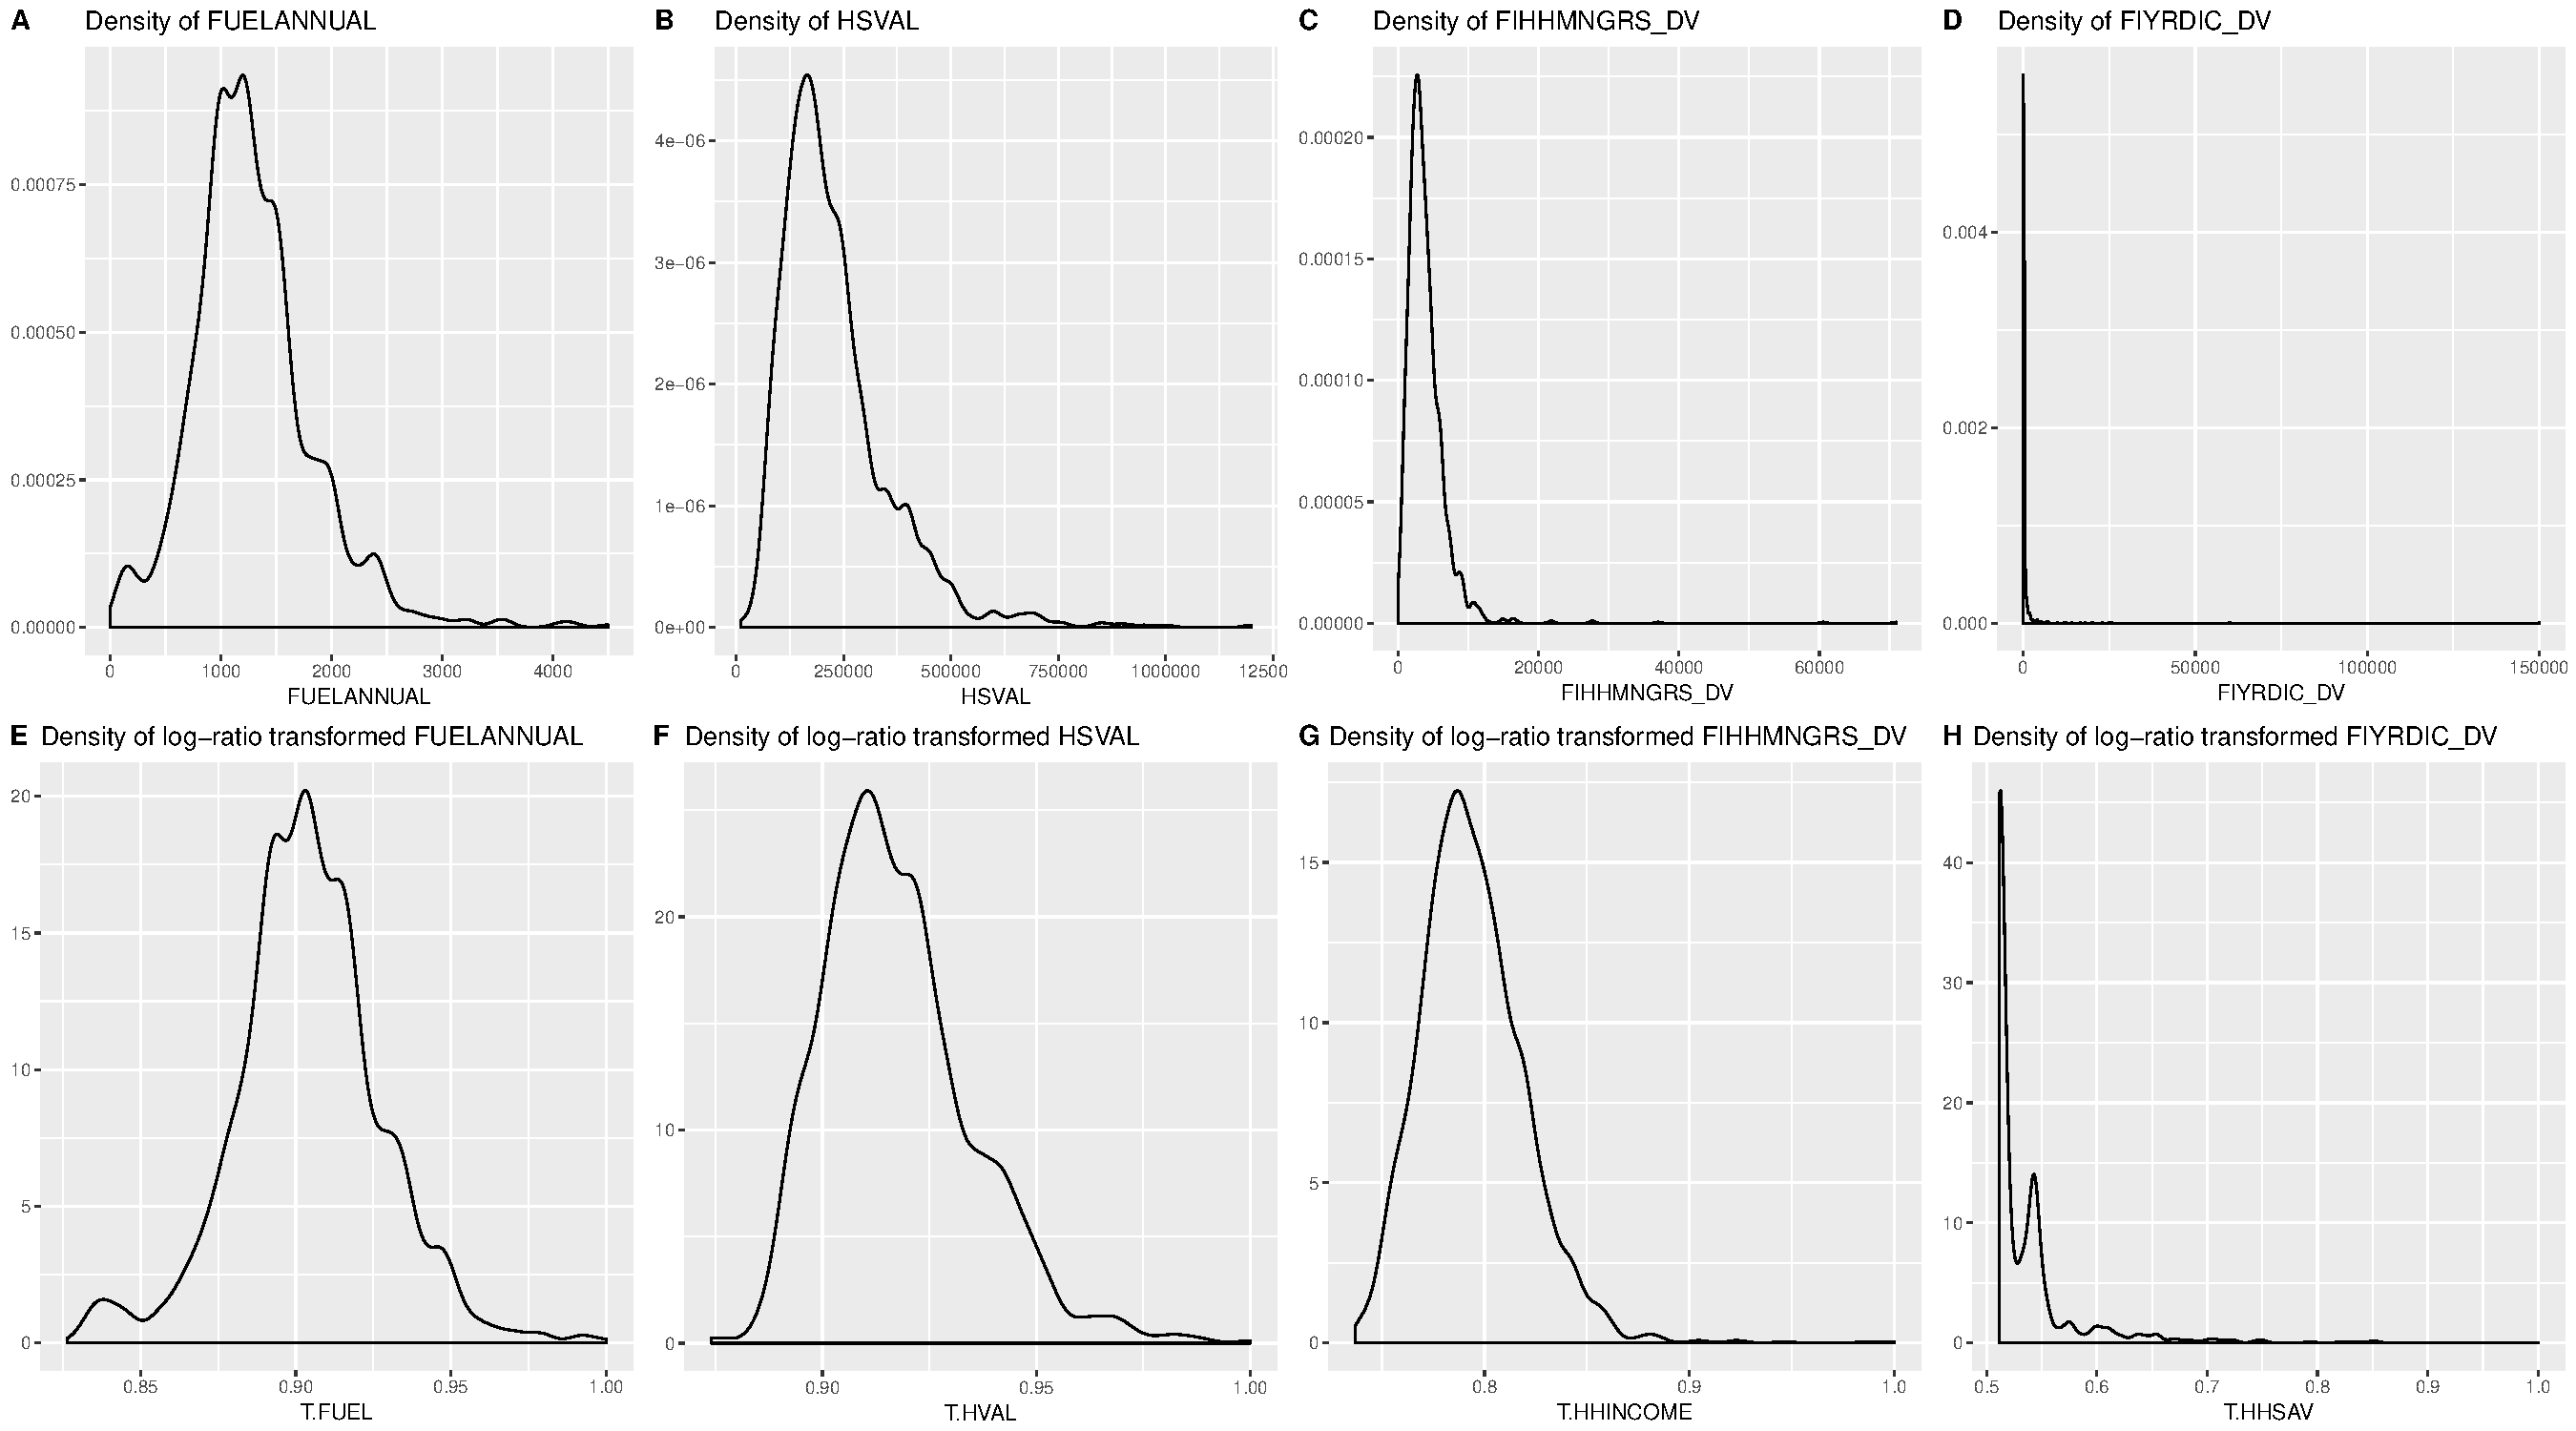
\includegraphics[width=17cm]{../Figure_logratio.pdf}
\end{center}
\caption{\footnotesize{Distributions of quantitative variables and log-ratio transformed}}
\label{Figure 2}
\end{figure}

After said correction, the distributions of the four stated variables were assessed as showed in figure 2A-D. The observation of a systematic skew towards increasing value lead to the use of a log-ratio transformation (offsetting by the mean), where:\\ 
$x=log(x+mean(log(x))/max(log(x+mean(log(x)))$,\\ 
producing the following variables: (i) $T.FUEL$, (ii) $T.HVAL$, (iii) $T.HHINCOME$, (iv) $T.HHSAV$.

The distribution of the first 3 are notably visibly improved (figure 2E-G). Additionally, in the process two unexpected ($.19.384765625$) values were identified in $FIHHMNGRS\_DV$. As non numerical, they were treated as missing and removed.

\subsection{Geographical data}
As mentioned earlier, one might assume that the climate and exterior temperature would highly influence heat necessity and consequently energy consumption. Based on the sole regional location of each household, I chose to use the centroid latitude of the region as a proxy for the climatic conditions. All the geographical data retrieved was initially from the \textit{Office of National Statistics and National Records Scotland data} as available here http://martinjc.github.io/UK-GeoJSON/.\\
From the data, the centroids latitude and longitude were computed ($LONG$, $LAT$) for each regions, as well as the number of samples per regions ($NSAMPLES$) and a dummy variable separating London from the rest. This additionally enables a visual representation of the survey, as seen in figure 2.

\begin{figure}[!h]
\begin{center}
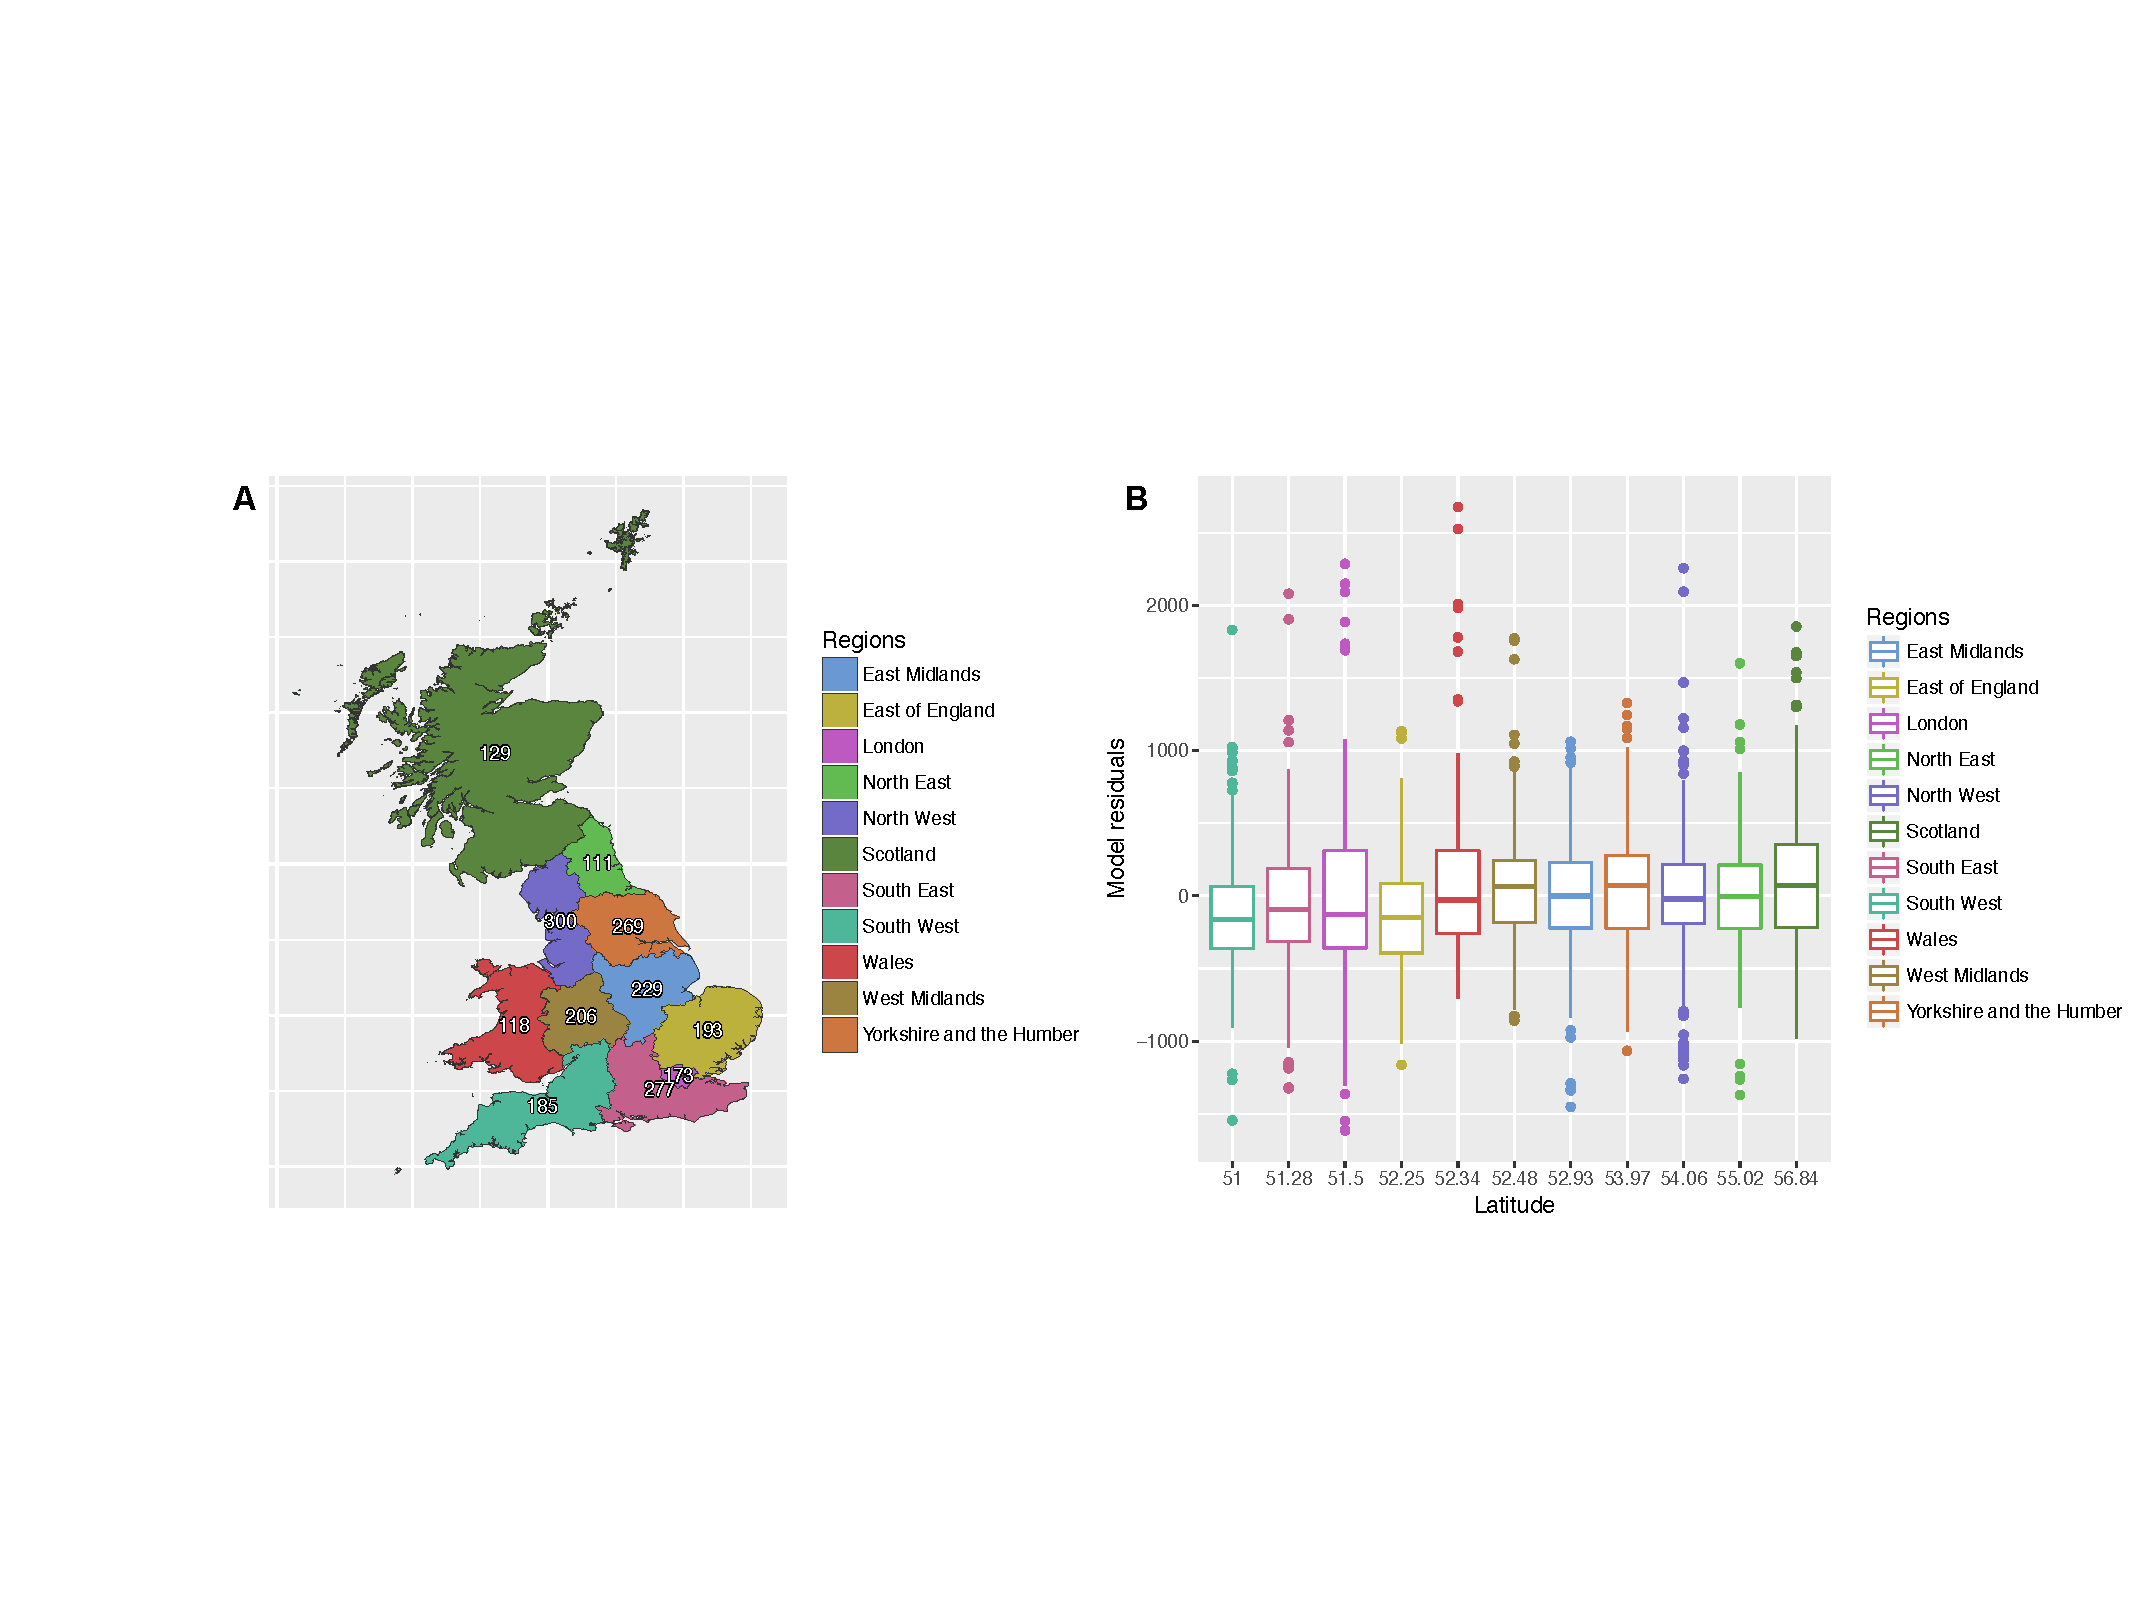
\includegraphics[width=17cm]{../Figure_map+lat.pdf}
\end{center}
\caption{\footnotesize{A - Map of the UK regions and countries with the number of respondents; B - Boxplot of FUELANNUAL depending on the latitude of the regions}}
\label{Figure 3}
\end{figure}

\subsection{Data encoding and transformation}
Firstly, some additional variables were computed based on the initial dataset. As such the $AGE$ was deducted from available data ($YEAR-BIRHTY$) and $REGION$ is just of nominal equivalent of $GOR\_DV$. Then the four geographical variables mentioned earlier as well as the four transformed variables, leading to the total number fo 43 variables.\\
Finally, as the last step each pre-selected variable was inspected and, if necessary, re-encoded in the appropriate data type, namely quantitative (<dbl> or <int>), ordinal (<ord>) or nominal (<fctr>). One can get a $glimpse()$ at the modified data structure, which will be the basis for the statistical analysis:\\
\begin{Answer}
\begin{verbatim}
Observations: 2,190
Variables: 43
\$ FUELANNUAL   <dbl> 1530, 1530, 480, 1360, 1800, 960, 735, 162...
\$ HSVAL        <dbl> 85000, 85000, 120000, 200000, 500000, 1750...
\$ GOR_DV       <dbl> 1, 1, 1, 1, 1, 1, 1, 1, 1, 1, 1, 1, 1, 1, ...
\$ YEAR         <dbl> 2011, 2011, 2011, 2011, 2011, 2011, 2011, ...
\$ HHSIZE       <dbl> 3, 3, 1, 1, 2, 2, 1, 4, 4, 4, 2, 2, 3, 3, ...
\$ HHTYPE_DV    <fctr> 3 or more adults, no children, incl. at l...
\$ HSBEDS       <dbl> 2, 2, 2, 4, 3, 3, 3, 3, 3, 3, 1, 1, 3, 3, ...
\$ TENURE_DV    <fctr> Owned with mortgage, Owned with mortgage,...
\$ NEMP_DV      <dbl> 2, 2, 0, 0, 0, 0, 0, 2, 2, 2, 2, 2, 2, 2, ...
\$ NKIDS_DV     <dbl> 0, 0, 0, 0, 0, 0, 0, 1, 1, 1, 0, 0, 0, 0, ...
\$ NPENS_DV     <dbl> 1, 1, 1, 1, 2, 1, 1, 0, 0, 0, 0, 0, 0, 0, ...
\$ NUE_DV       <dbl> 1, 1, 1, 1, 2, 2, 1, 1, 1, 1, 0, 0, 1, 1, ...
\$ LKMOVE       <fctr> Wants to stay, Wants to move, Wants to mo...
\$ XPMOVE       <fctr> Not expecting to move, Not expecting to m...
\$ FIHHMNGRS_DV <dbl> 1933.330, 1933.330, 1152.000, 990.016, 187...
\$ FIYRDIC_DV   <dbl> 0.0000, 0.0000, 0.0000, 138.1658, 138.1658...
\$ FINNOW       <ord> 3, 2, 1, 2, 3, 3, 2, 2, 2, 2, 4, 3, 3, 3, ...
\$ FINFUT       <ord> 3, 3, 3, 3, 3, 1, 3, 2, 3, 1, 1, 2, 3, 3, ...
\$ SAVE         <fctr> No monthly savings, Monthly savings, Mont...
\$ JBSTAT       <fctr> Retired, In paid employment (full or part...
\$ SF1          <ord> 2, 1, 3, 4, 5, 3, 1, 2, 4, 2, 2, 2, 2, 4, ...
\$ RACEL_DV     <fctr> British/English/Scottish/Welsh/Northern I...
\$ BIRTHY       <dbl> 1949, 1975, 1937, 1928, 1944, 1948, 1947, ...
\$ SEX          <fctr> Female, Female, Female, Female, Female, F...
\$ NCARS        <dbl> 2, 2, 1, 0, 1, 2, 1, 2, 2, 2, 3, 3, 1, 1, ...
\$ ENVHABIT1_A  <ord> 1, 1, 4, 5, 5, 5, 5, 1, 1, 1, 2, 4, 5, 5, ...
\$ ENVHABIT3_A  <ord> 1, 1, 4, 5, 2, 1, 5, 5, 5, 5, 4, 3, 5, 1, ...
\$ ENVHABIT4_A  <ord> 4, 1, 3, 4, 4, 5, 5, 4, 3, 3, 4, 4, 5, 5, ...
\$ ENVHABIT6_A  <ord> 1, 3, 4, 3, 3, 3, 4, 4, 3, 1, 1, 1, 1, 4, ...
\$ ENVHABIT8_A  <ord> 1, 1, 1, 1, 2, 1, 1, 0, 1, 2, 2, 1, 3, 1, ...
\$ FUELDUEL     <fctr> Separate, Separate, Separate, One bill, O...
\$ HEATCH       <fctr> Some form of central heating, Some form o...
\$ HHEAT        <fctr> Yes, Yes, Yes, Yes, Yes, No, Yes, Yes, Ye...
\$ AGE          <dbl> 62, 36, 74, 83, 67, 63, 64, 49, 61, 18, 59...
\$ REGION       <fctr> North East, North East, North East, North...
\$ LONDON       <fctr> Not London, Not London, Not London, Not L...
\$ LAT          <dbl> 55.01955, 55.01955, 55.01955, 55.01955, 55...
\$ LONG         <dbl> -1.905265, -1.905265, -1.905265, -1.905265...
\$ NSAMPLES     <int> 111, 111, 111, 111, 111, 111, 111, 111, 11...
\$ T.FUEL       <dbl> 0.9169092, 0.9169092, 0.8630868, 0.9097256...
\$ T.HVAL       <dbl> 0.8932624, 0.8932624, 0.9006958, 0.9152191...
\$ T.HHINCOME   <dbl> 0.7726595, 0.7726595, 0.7598525, 0.7569503...
\$ T.HHSAV      <dbl> 0.5117663, 0.5117663, 0.5117663, 0.5343909...
\end{verbatim}
\end{Answer}


\section{Model Selection and Evaluation}
\subsection{Significant variables}
After a careful inspection as well as a normative pre-selection based on their characteristics and meaningfulness, variables were tested for their relationship with the response variable, proxy for the energy consumption. The statistical analysis was performed (1) on the non-transformed variables, (2) then adding the geographical parameters, (3) introducing the transformed variables instead of the non-transformed and (4) investigating matters related to London\\

The first approached used was to build linear models within in variable category (e.g. $Economics$) and identify the relevant subset of variables.  In addition of the response variable and the housing wealth, this process identified 13 explanatory variables: $NCARS$, $ENVHABIT1_A$, $ENVHABIT8_A$, $SAVE$, $T.HHINCOME$, $FINNOW$, $FIYRDIC_DV$, $RACEL_DV$, $AGE$, $HHTYPE_DV$, $HSBEDS$, $TENURE_DV$, $FUELDUEL$.\\
 
In addition of this method, the possibility of creating indexes through clustering variables within each category was investigated as follows:\\
\begin{enumerate}
\item Significant variables from each category were used to compute the Gower distances between observations.
\item The distance matrix was clustered (Partitioning Around Medoids - PAM) after an estimation of the optimal number of clusters.
\item The category, now transformed into a nominal variable, was tested against $FUELANNUAL$ in a linear model.\\
\end{enumerate}

Figure 4A illustrates the two clusters identified in the $Environmental$ variables category. However, if such method can synthesise a lot of information and reduce de dimensionality of the data, using the clusters was less performant than the initial variables in all categories.\\

The 13 variables previously identified were used to build a first comprehensive model. Due to the number of variables at stake, I arbitrarily choose not to investigate potential interactions between said variables. Specific interactions, however, will be investigated in two cases on subsequent models. A two-directional AIC optimisation was performed to identify the relevant combination of the 13 variables. Sanity checks were performed, and the variables significance was then confirmed by a type II anova.

\begin{Answer}
\begin{verbatim}
Anova Table (Type II tests)

Response: FUELANNUAL
               Sum Sq   Df F value    Pr(>F)    
HSVAL        17927176    1 76.4401 < 2.2e-16 ***
HHTYPE_DV    41165995   16 10.9705 < 2.2e-16 ***
HSBEDS        7893932    1 33.6591 7.536e-09 ***
TENURE_DV     3289861    4  3.5069  0.007331 ** 
FINNOW        2465511    4  2.6282  0.032907 *  
SAVE          1430809    1  6.1009  0.013589 *  
ENVHABIT1_A   8749943    5  7.4618 5.947e-07 ***
FUELDUEL     12793049    1 54.5485 2.156e-13 ***
AGE           1520098    1  6.4816  0.010969 *  
Residuals   505403393 2155                      
---
Signif. codes:  0 ‘***’ 0.001 ‘**’ 0.01 ‘*’ 0.05 ‘.’ 0.1 ‘ ’ 1
\end{verbatim}
\end{Answer}

The type II anova reports the sum of square, and therefore the amount of variable explained by the variable (as compared to the Residuals), the degrees of freedom (Df) and the significance (p-value on the F statistic). Note that the significance threshold used throughout the analysis is $\alpha = 0.05$.\\

The former anova table corresponds to the following model:

\begin{Answer}
\begin{verbatim}
Call:
lm(formula = FUELANNUAL ~ HSVAL + HHTYPE_DV + HSBEDS + TENURE_DV + 
    FINNOW + SAVE + ENVHABIT1_A + FUELDUEL + AGE, data = data.correct)

Residuals:
     Min       1Q   Median       3Q      Max 
-1614.58  -273.31   -42.83   225.94  2674.74 

[...]

Residual standard error: 484.3 on 2155 degrees of freedom
Multiple R-squared:  0.2398,	Adjusted R-squared:  0.2278 
F-statistic: 19.99 on 34 and 2155 DF,  p-value: < 2.2e-16

[...]

	studentized Breusch-Pagan test

data:  lm.red
BP = 182.18, df = 34, p-value < 2.2e-16
\end{verbatim}
\end{Answer}

Interestingly, the model is highly significant and the adjusted $R^2$ is roughly 22.8\%. However, the studentized Breusch-Pagan test indicates a significant heteroskedasticity, which I will try to address in the following models.

\subsection{Geographical variables}

The previous model does account for most of the categories stated in the introduction. However, the regional and climatic conditions are not yet accounted for. The subsequent model therefore introduces the latitude as an explanatory variable (I acknowledge that directly using the nominal variable $REGION$ could have brought similar insights, but doesn't introduce the quantitive latitudinal gradient).

\begin{Answer}
\begin{verbatim}
Call:
lm(formula = FUELANNUAL ~ HSVAL + HHTYPE_DV + HSBEDS + TENURE_DV + 
    FINNOW + SAVE + ENVHABIT1_A + FUELDUEL + AGE + LAT, data = data.correct)

Residuals:
     Min       1Q   Median       3Q      Max 
-1570.78  -280.08   -33.19   233.29  2685.57 

[...]

Residual standard error: 481.7 on 2154 degrees of freedom
Multiple R-squared:  0.2481,	Adjusted R-squared:  0.2359 
F-statistic: 20.31 on 35 and 2154 DF,  p-value: < 2.2e-16
\end{verbatim}
\end{Answer}

Latitude indeed is a significant explanatory variable ($p-value = 1.049e^{-06}$, type II anova). Its effects can be captured in table 1, along with the ones of other explanatory variables.\\

\begin{table}[]
\centering
\caption{Partial summary of the linear model including latitude (missing $HHTYPE\_DV$)}
\label{Table 1}
\begin{tabular}{llllll}
 & Estimate                                                                        & Std. Error & t value   & Pr(\textgreater|t|) &     \\
\hline
(Intercept)                                                                     & -1.954e+03 & 4.006e+02 & -4.876              & 1.16e-06       & *** \\
HSVAL                                                                           & 8.925e-04  & 9.240e-05 & 9.660               & \textless2e-16 & *** \\
...                                                                      & ... & ... & ... & ... & ...\\
HSBEDS                                                                          & 8.431e+01  & 1.481e+01 & 5.692               & 1.43e-08       & *** \\
TENURE\_DVLocal authority rent                                                  & -2.420e+02 & 5.080e+02 & -0.476              & 0.633894       &     \\
TENURE\_DVOwned outright                                                        & 4.067e+02  & 1.389e+02 & 2.929               & 0.003435       & **  \\
TENURE\_DVOwned with mortgage                                                   & 4.328e+02  & 1.373e+02 & 3.152               & 0.001646       & **  \\
TENURE\_DVRented private unfurnished                                            & 5.694e+02  & 5.035e+02 & 1.131               & 0.258196       &     \\
FINNOW.L                                                                        & 7.576e+01  & 5.280e+01 & 1.435               & 0.151476       &     \\
FINNOW.Q                                                                        & 5.559e+01  & 4.430e+01 & 1.255               & 0.209688       &     \\
FINNOW.C                                                                        & -5.011e+01 & 3.725e+01 & -1.345              & 0.178746       &     \\
FINNOW\textasciicircum 4                                                        & -2.403e+01 & 2.791e+01 & -0.861              & 0.389435       &     \\
SAVENo monthly savings                                                          & 4.912e+01  & 2.223e+01 & 2.210               & 0.027236       & *   \\
ENVHABIT1\_A.L                                                                  & -1.418e+02 & 6.333e+01 & -2.239              & 0.025258       & *   \\
ENVHABIT1\_A.Q                                                                  & 2.001e+01  & 6.089e+01 & 0.329               & 0.742518       &     \\
ENVHABIT1\_A.C                                                                  & -1.724e+01 & 4.709e+01 & -0.366              & 0.714370       &     \\
ENVHABIT1\_A\textasciicircum 4                                                  & 5.831e+00  & 3.745e+01 & 0.156               & 0.876308       &     \\
ENVHABIT1\_A\textasciicircum 5                                                  & 1.841e+01  & 3.825e+01 & 0.481               & 0.630369       &     \\
FUELDUELSeparate                                                                & 1.616e+02  & 2.107e+01 & 7.668               & 2.62e-14       & *** \\
AGE                                                                             & 2.466e+00  & 9.416e-01 & 2.618               & 0.008895       & **  \\
LAT                                                                             & 3.462e+01  & 7.072e+00 & 4.896               & 1.05e-06       & *** \\
\hline
\end{tabular}
\end{table}

The summary table of the linear models enables to interpret the effect of each explanatory variable. Firstly the significance of the explanatory variable is reported by the p-value. However, it is important to highlight that comparing a specific category of a nominal or ordinal variable to the intercept might be significant, despite the overall variable being significant (e.g. the reported categories of $FINNOW$ hereby reported do not appear as significant, whereas a type II anova indicates a p-value of $0.031368$).\\
In addition of significance, the table reports the estimate, which is the estimated parameter of the linear relationship. In a linear model $Y_i = \mu + \beta X_i+ E_{i}$ with $ E_{i} \sim \mathcal{N}(0,\sigma^2)$, $\mu$ would be the intercept and $\beta$ the estimate for the quantitative explanatory variable $X$. Assuming $X$ is $LAT$, from the previous table we have $\mu = -1.954e^{03}$ and $\beta = 3.462e^{01}$.\\

This effect of the latitude can be represented based on the residuals from the former model (Figure 3B). Despite being weak, the increase of consumption does follow the increase in latitude, apart from London which seems to be behaving differently.\\

\begin{figure}[!h]
\begin{center}
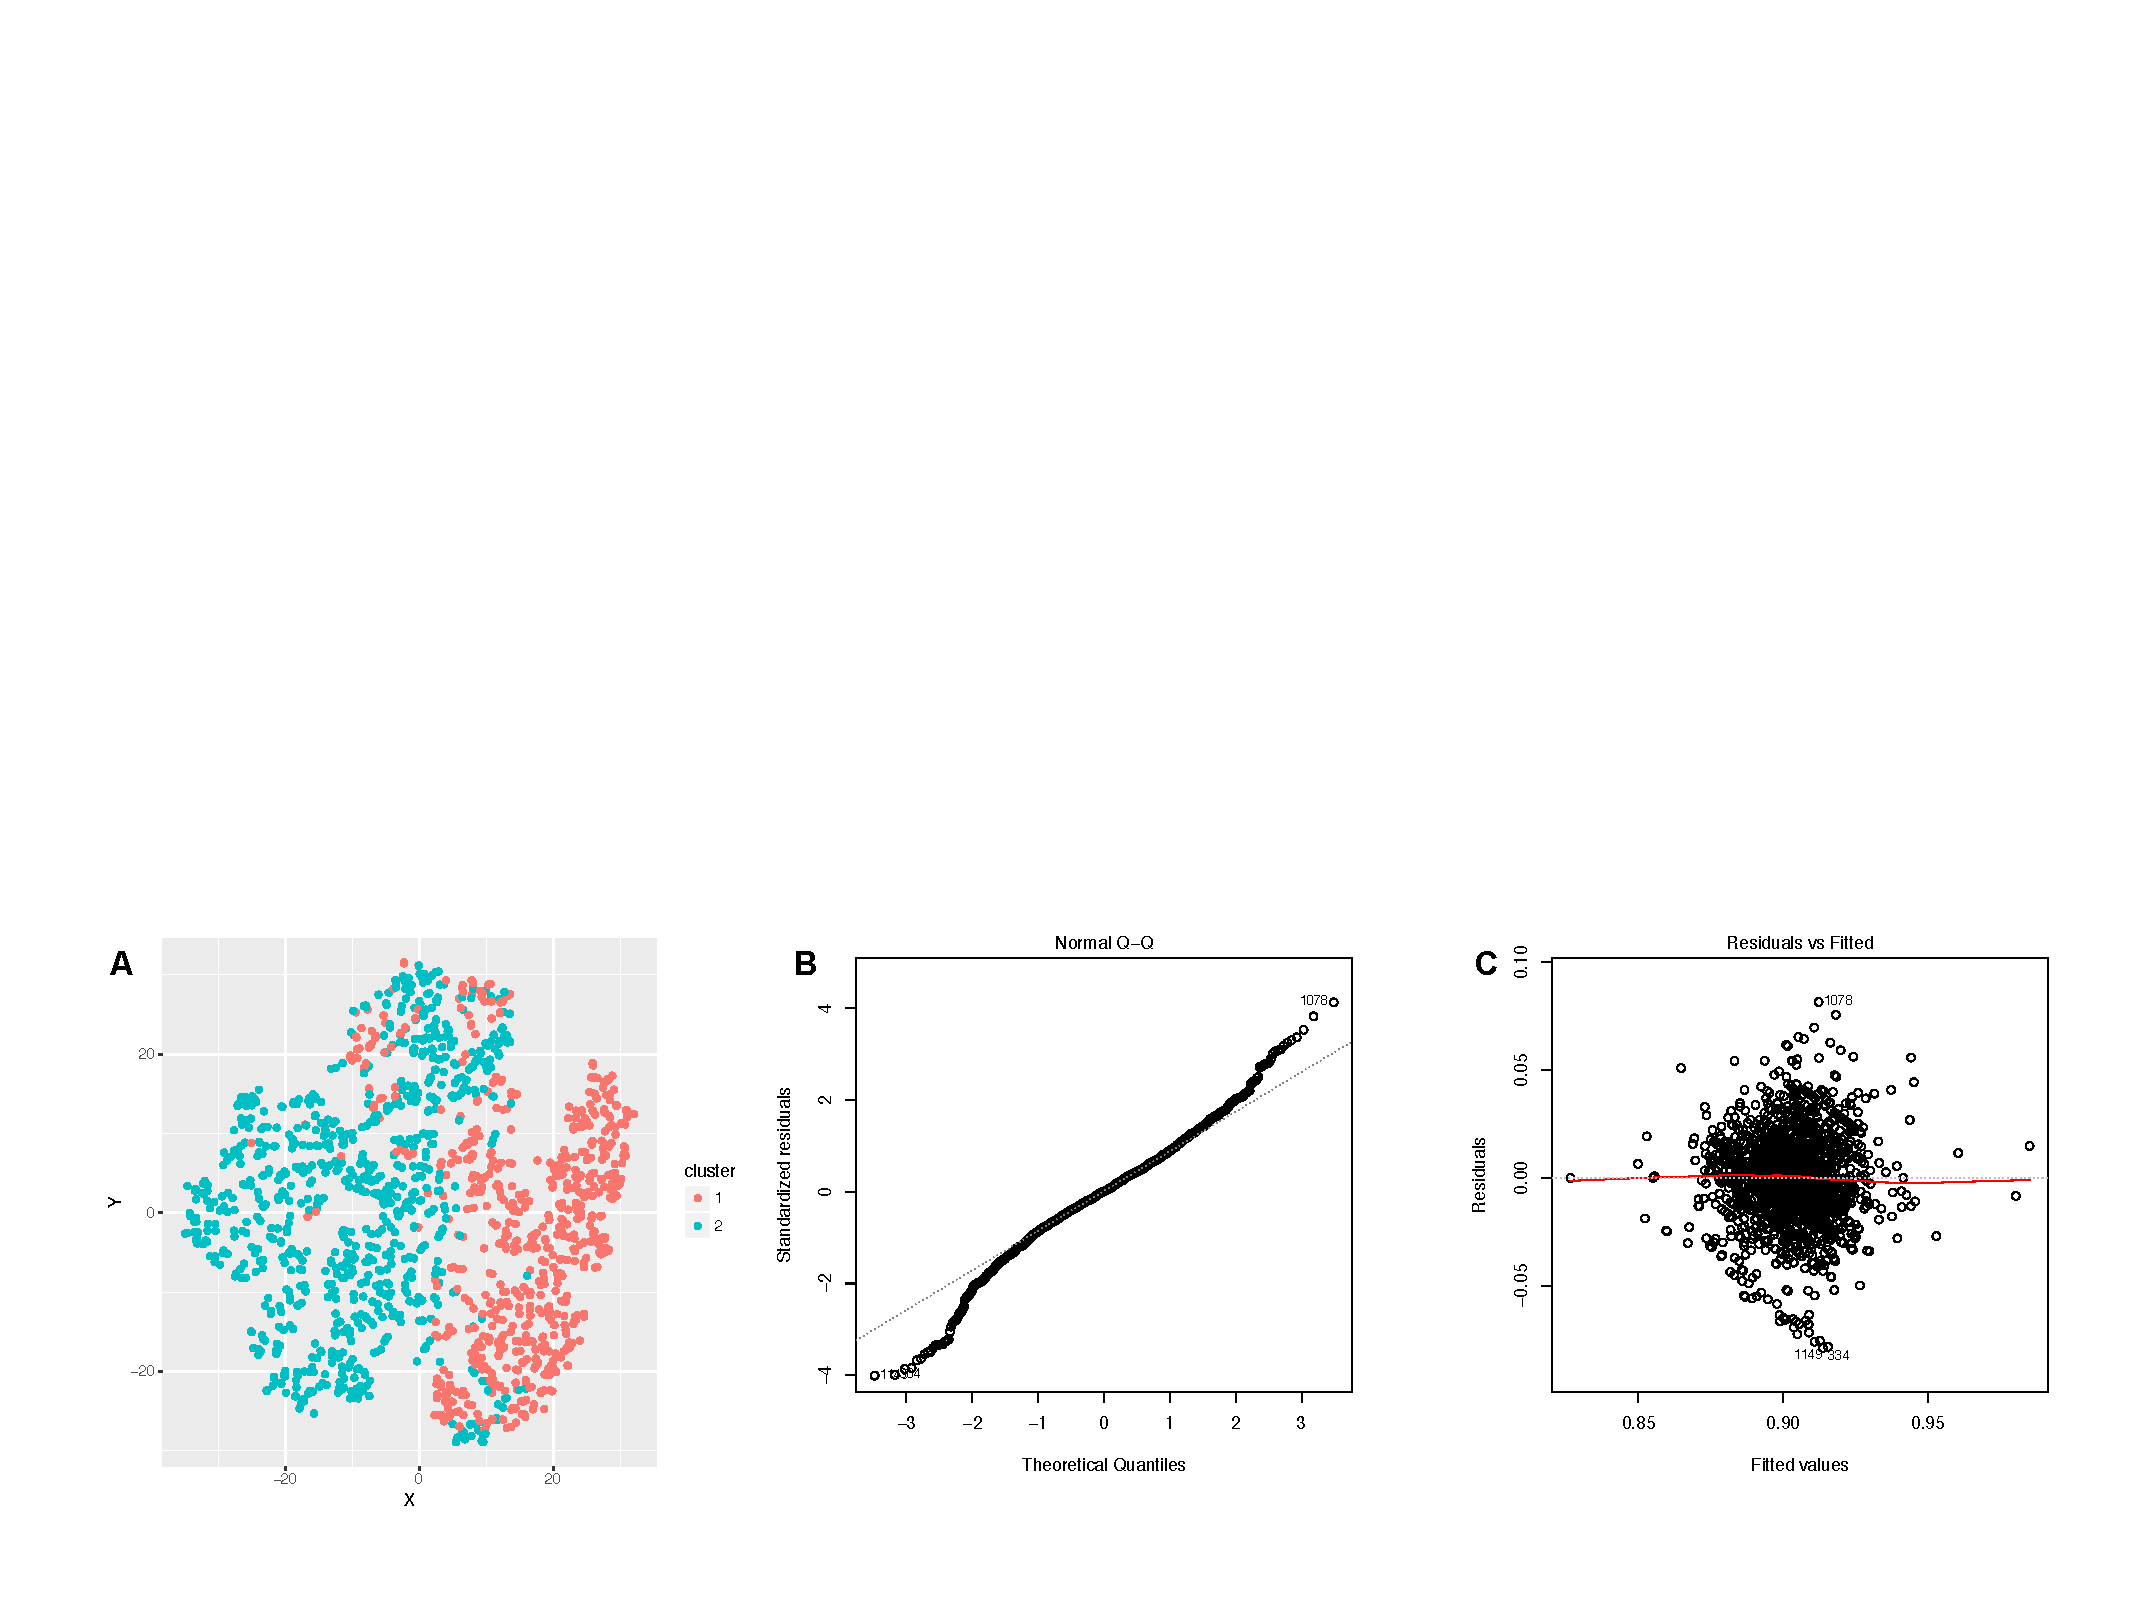
\includegraphics[width=17cm]{../Figure_clust+diagnostic.pdf}
\end{center}
\caption{\footnotesize{A - Figure of the clustered environmental variables. Represented in t-SNE reduced space ; Diagnostic plot of the last model (B - QQplot and C - Residuals vs Fitted)}}
\label{Figure 4}
\end{figure}

\subsection{Log-Ration relationships}

However, transforming the quantitative variables using a log-ratio improved the normality of the distributions. Consequently, this part will investigate the effect of transforming the quantitative variables on the previous model.\\

\begin{Answer}
\begin{verbatim}
Call:
lm(formula = T.FUEL ~ HSVAL + HHTYPE_DV + HSBEDS + TENURE_DV + 
    T.HHINCOME + FINNOW + SAVE + RACEL_DV + NCARS + 
    ENVHABIT1_A + FUELDUEL + AGE + LAT, data = data.correct)
    
[...]

Residual standard error: 0.02086 on 2131 degrees of freedom
  (8 observations deleted due to missingness)
Multiple R-squared:  0.2577,	Adjusted R-squared:  0.2403 
F-statistic:  14.8 on 50 and 2131 DF,  p-value: < 2.2e-16
\end{verbatim}
\end{Answer}

The improvement was not highly consequential, though the model's adjusted $R^2$ is now of 24\%. Nevertheless, if far from being removed, the heteroskedasticity formerly observed was reduced by the transformation.

\subsection{London and the other regions}

As seen previously, we noticed the particular behaviour of London. As such, a variable $LONDON$, representing either London or the other regions, was introduced in the model as an interaction with all the other variables.\\

\begin{Answer}
\begin{verbatim}
Call:
lm(formula = T.FUEL ~ LONDON * (HSVAL + HHTYPE_DV + HSBEDS + 
    TENURE_DV + T.HHINCOME + FINNOW + SAVE + RACEL_DV + NCARS + 
    FIHHMNGRS_DV + ENVHABIT1_A + FUELDUEL + AGE + LAT), data = data.correct)

[...]

Residual standard error: 0.02037 on 2088 degrees of freedom
  (8 observations deleted due to missingness)
Multiple R-squared:  0.3068,	Adjusted R-squared:  0.2759 
F-statistic: 9.936 on 93 and 2088 DF,  p-value: < 2.2e-16
\end{verbatim}
\end{Answer}

The introduction of the variable and its interactions was of indeed significant and also increased the overall explanatory power of the model. To investigate this result further, the dataset was subsequently split into the data from London and the data from the rest of the UK.\\

A similar process as what was described in 3.1 was conducted and this allowed to build (1) a totally model for London and (2) revise the results on the rest of the UK, with the additional inclusion of geographical and transformed variables.\\

\begin{Answer}
\begin{verbatim}
Anova Table (Type II tests)

Response: T.FUEL
              Sum Sq  Df F value    Pr(>F)    
HHTYPE_DV   0.055742  14  7.2457 2.171e-11 ***
SAVE        0.003232   1  5.8807   0.01648 *  
ENVHABIT1_A 0.005563   5  2.0249   0.07820 .  
Residuals   0.083526 152      

[...]

Call:
lm(formula = T.FUEL ~ HHTYPE_DV + SAVE + ENVHABIT1_A, data = data.london)

Residual standard error: 0.02344 on 152 degrees of freedom
Multiple R-squared:  0.4785,	Adjusted R-squared:  0.4098 
F-statistic: 6.972 on 20 and 152 DF,  p-value: 2.018e-13

[...]

	studentized Breusch-Pagan test

data:  lm.london.red
BP = 45.026, df = 20, p-value = 0.001095
\end{verbatim}
\end{Answer}     

The latter model is notable in 4 main ways. First, the number of explanatory variables has massively decreased, $HHTYPE\_DV$ being from far the most relevant. Secondly, the adjusted $R^2$ reached roughly 41\% and, thirdly, if still significant on using a studentized Breusch-Pagan test, the heteroskedasticity is almost removed. Finally, probably the most interesting result is that the housing wealth effect ($HSVAL$) is not significant in London.\\

The similar process was realised for the rest of the UK, with the addition of potential interaction between $HSVAL$, the explanatory variable of interest, and other explanatory variables. This leads to the following (and final) model:

\begin{Answer}
\begin{verbatim}
Call:
lm(formula = T.FUEL ~ HSVAL * (HHTYPE_DV + HSBEDS + TENURE_DV + 
    FINNOW + RACEL_DV + NCARS + ENVHABIT1_A + FUELDUEL + AGE + 
    LAT + T.HHINCOME), data = data.not.london)

[...]
    
Residual standard error: 0.02 on 1919 degrees of freedom
  (5 observations deleted due to missingness)
Multiple R-squared:  0.2986,	Adjusted R-squared:  0.265 
F-statistic: 8.882 on 92 and 1919 DF,  p-value: < 2.2e-16

[...]

	studentized Breusch-Pagan test

data:  lm.nlon.red.int
BP = 138.34, df = 92, p-value = 0.001283
\end{verbatim}
\end{Answer} 

Interestingly, the model remains quite similar to the ones built on the overall dataset. $HSVAL$ does indeed have some significant interactions (for example with $HHTYPE\_DV$), which can be formalised as follows:\\

$Y_{ij} = \mu + \alpha_i + \beta X_{ij} + \gamma_i X_{ij} +  E_{i}$ with $ E_{ij} \sim \mathcal{N}(0,\sigma^2)$, $i$ the categories of $HTTYPE\_DV$ and $j$ the observations.\\

This can be interpreted as $\alpha_i$ being the mean of each category, $\beta$ the slope of the $Y \sim X$ relationship and $\gamma_i$ the deviation of that slope, for each category.\\

Notably, the model estimates $\beta = -6.565e^{-07}$ and $\gamma_i = 1.420e^{-07}$ for $i$ being "1 adult, 1 child". Which does not go in the direction of a general housing wealth effect in the rest of the UK either.\\

Moreover, similarly to the model designed for London, heteroskedasticity is highly reduced. Particularly, when looking at the diagnostic plots (see figure 4B and C), I argue that if there still is some issues on the \textit{QQPlot} as the absolute values increase, the \textit{Residuals vs Fitted} plot does not show much deviation from 0.

\section{Empirical Findings and Discussions}

If the results have already bee commented through the models constructions and evaluation, this section will provide a synthesis and further interpretation. Firstly, the evolution of the models shows three main influences:\\

\begin{enumerate}
\item log-ratio transformation of the quantitative variables were beneficial for the linear regression, particularly conrcerning $FUELANNUAL$ ($T.FUEL$), the response variable, and $FIHHMNGRS$ ($T.HHINCOME$).
\item The mean latitude of the region, which is likely to be a proxy for climatic conditions does influence energy consumption
\item London and the rest of the UK display two very different behaviours, leading to the construction of two very different models. \\
\end{enumerate}

In the case of London, the remaining explanatory variables were $HHTYPE\_DV$ (the structure of the household), $SAVE$ (whether people are able to save money monthly) and $ENVHABIT1\_A$ (how often do people leave the tv on standby for the night), which would be representative of the categories $Household$, $Economics$ and $Environmental$.\\

For the rest of the UK, the main explanatory variables were $HSVAL$, $HHTYPE\_DV$, $HSBEDS$, $TENURE\_DV$, $FINNOW$, $RACEL\_DV$, $NCARS$, $ENVHABIT1\_A$, $FUELDUEL$, $AGE$, $LAT$, $T.HHINCOME$.
Said variables can be ordered as follow:
\begin{enumerate}
\item $Dynamics$: $LAT$
\item $Household$: $HHTYPE\_DV$, $HSBEDS$, $TENURE\_DV$
\item $Economics$: $FINNOW$, $T.HHINCOME$
\item $Cultural$: $AGE$, $RACEL\_DV$
\item $Environmental$: $NCARS$, $ENVHABIT1\_A$
\item $Fuel \& Heating$: $FUELDUEL$ \\
\end{enumerate}

This tends to confirm the complexe and multifactorial nature of energy consumption that had been identified (Jones et al., 2015). The large number of observations and there even distribution across regions and working status (roughly 2 thirds employed, a third retired and the rest) gives statistical strength to the results. Additionally the possibility to correct for a wide variety of factors, from cultural to economical enables to capture the complexity of the explanatory variables. However, the number of variable that could be tested did not enable some key hypothesis, such as the influence of electrical appliance or the actual size of of the house in square meters. In addition, if greatly reduced, the heteroskedasticity might still be an issue to the robustness of the models.\\

Finally, taking into account the limits of the analysis, results nevertheless suggest a weak if not inexistent housing wealth effect on energy consumption in the UK. Indeed, in the case of London, the housing wealth was not identified as a significant explanatory variable at all. For the rest of the UK, the situation is slightly more complicated. As explicated in part 3.4, the final model does attest for a significant role of housing effect. However, if in a non interactive mode, the estimate would be $3.348e^{-08}$, housing wealth can be involved various interactions which can lead to negative wealth effects in some cases. In any case, the general trend remains a positive but the dedicated $R^2$ is low (3,7\% out of the 29.9\% from the last model).

\section{Bibliography}
\begin{enumerate}

\item Buiter, W. H. (2008). Housing wealth isn't wealth (No. w14204). National Bureau of Economic Research.

\item Calomiris, C., Longhofer, S. D., \& Miles, W. (2009). The (mythical?) housing wealth effect (No. w15075). National Bureau of Economic Research.

\item Carroll, C. D., Otsuka, M., \& Slacalek, J. (2011). How large are housing and financial wealth effects? A new approach. Journal of Money, Credit and Banking, 43(1), 55-79.

\item Case, K. E., Quigley, J. M., \& Shiller, R. J. (2005). Comparing wealth effects: the stock market versus the housing market. Advances in macroeconomics, 5(1).

\item Jones, R. V., Fuertes, A., \& Lomas, K. J. (2015). The socio-economic, dwelling and appliance related factors affecting electricity consumption in domestic buildings. Renewable and Sustainable Energy Reviews, 43, 901-917.

\end{enumerate}

\end{document}






